\documentclass[a4paper]{article}

\usepackage{eurosym}
\usepackage[utf8]{inputenc}
\usepackage[portuguese]{babel}
\usepackage{a4wide}
\usepackage[hyphens]{url}
\usepackage[hidelinks]{hyperref}
\usepackage{graphicx}
\usepackage{wrapfig}
\usepackage{amsmath}
\usepackage{verbatim}
\usepackage{caption}
\usepackage{subcaption}
\usepackage{float}
\usepackage{listings} 
\usepackage{ulem}
\usepackage{fancyvrb}
\usepackage[table,xcdraw]{xcolor}
\usepackage{comment}
\usepackage{indentfirst}
\usepackage{longtable}
\usepackage{subfiles}
\usepackage[bottom]{footmisc}
\usepackage{color,soul}
\usepackage{pdflscape}
\usepackage{multirow}

\setlength{\footskip}{20pt}
\DeclareUnicodeCharacter{20AC}{\euro}

\graphicspath{{images/}{../images/}}

\definecolor{codegreen}{rgb}{0,0.6,0}
\definecolor{codegray}{rgb}{0.5,0.5,0.5}
\definecolor{codepurple}{rgb}{0.58,0,0.82}
\definecolor{backcolour}{rgb}{0.95,0.95,0.92}
\definecolor{white}{rgb}{1,1,1}

\lstdefinestyle{mystyle}{
    backgroundcolor=\color{backcolour},   
    commentstyle=\color{codegreen},
    keywordstyle=\color{magenta},
    numberstyle=\tiny\color{codegray},
    stringstyle=\color{codepurple},
    basicstyle=\footnotesize,
    breakatwhitespace=false,         
    breaklines=true,                 
    captionpos=b,                    
    keepspaces=true,                 
    numbers=left,                    
    numbersep=5pt,                  
    showspaces=false,                
    showstringspaces=false,
    showtabs=false,                  
    tabsize=2
}
 
\lstset{style=mystyle}

\makeatletter
\renewcommand\paragraph{\@startsection{paragraph}{4}{\z@}%
            {-2.5ex\@plus -1ex \@minus -.25ex}%
            {1.25ex \@plus .25ex}%
            {\normalfont\normalsize\bfseries}}
\makeatother
\setcounter{secnumdepth}{4} % how many sectioning levels to assign numbers to
\setcounter{tocdepth}{4}    % how many sectioning levels to show in ToC



\begin{document}
\begin{titlepage}
\begin{center}



\includegraphics[width=0.6\textwidth]{images/logo.jpg}\\[0.5cm]

{\large Universidade do Minho - Escola de Engenharia}\\[0.5cm]

{\large Engenharia de Aplicações}\\[0.8cm]

% Title
\rule{\linewidth}{0.5mm} \\[0.4cm]
{ \huge \bfseries Aplicação \textit{Home4All}\\[0.4cm] }
\rule{\linewidth}{0.5mm} \\[1.5cm]

% Author and supervisor
\noindent
\begin{minipage}{0.5\textwidth}
  \begin{center} \large
    \textit{Autores:}\\[0.3cm]
  \end{center}
  \begin{flushleft} \large
    $ \begin{array}{l} 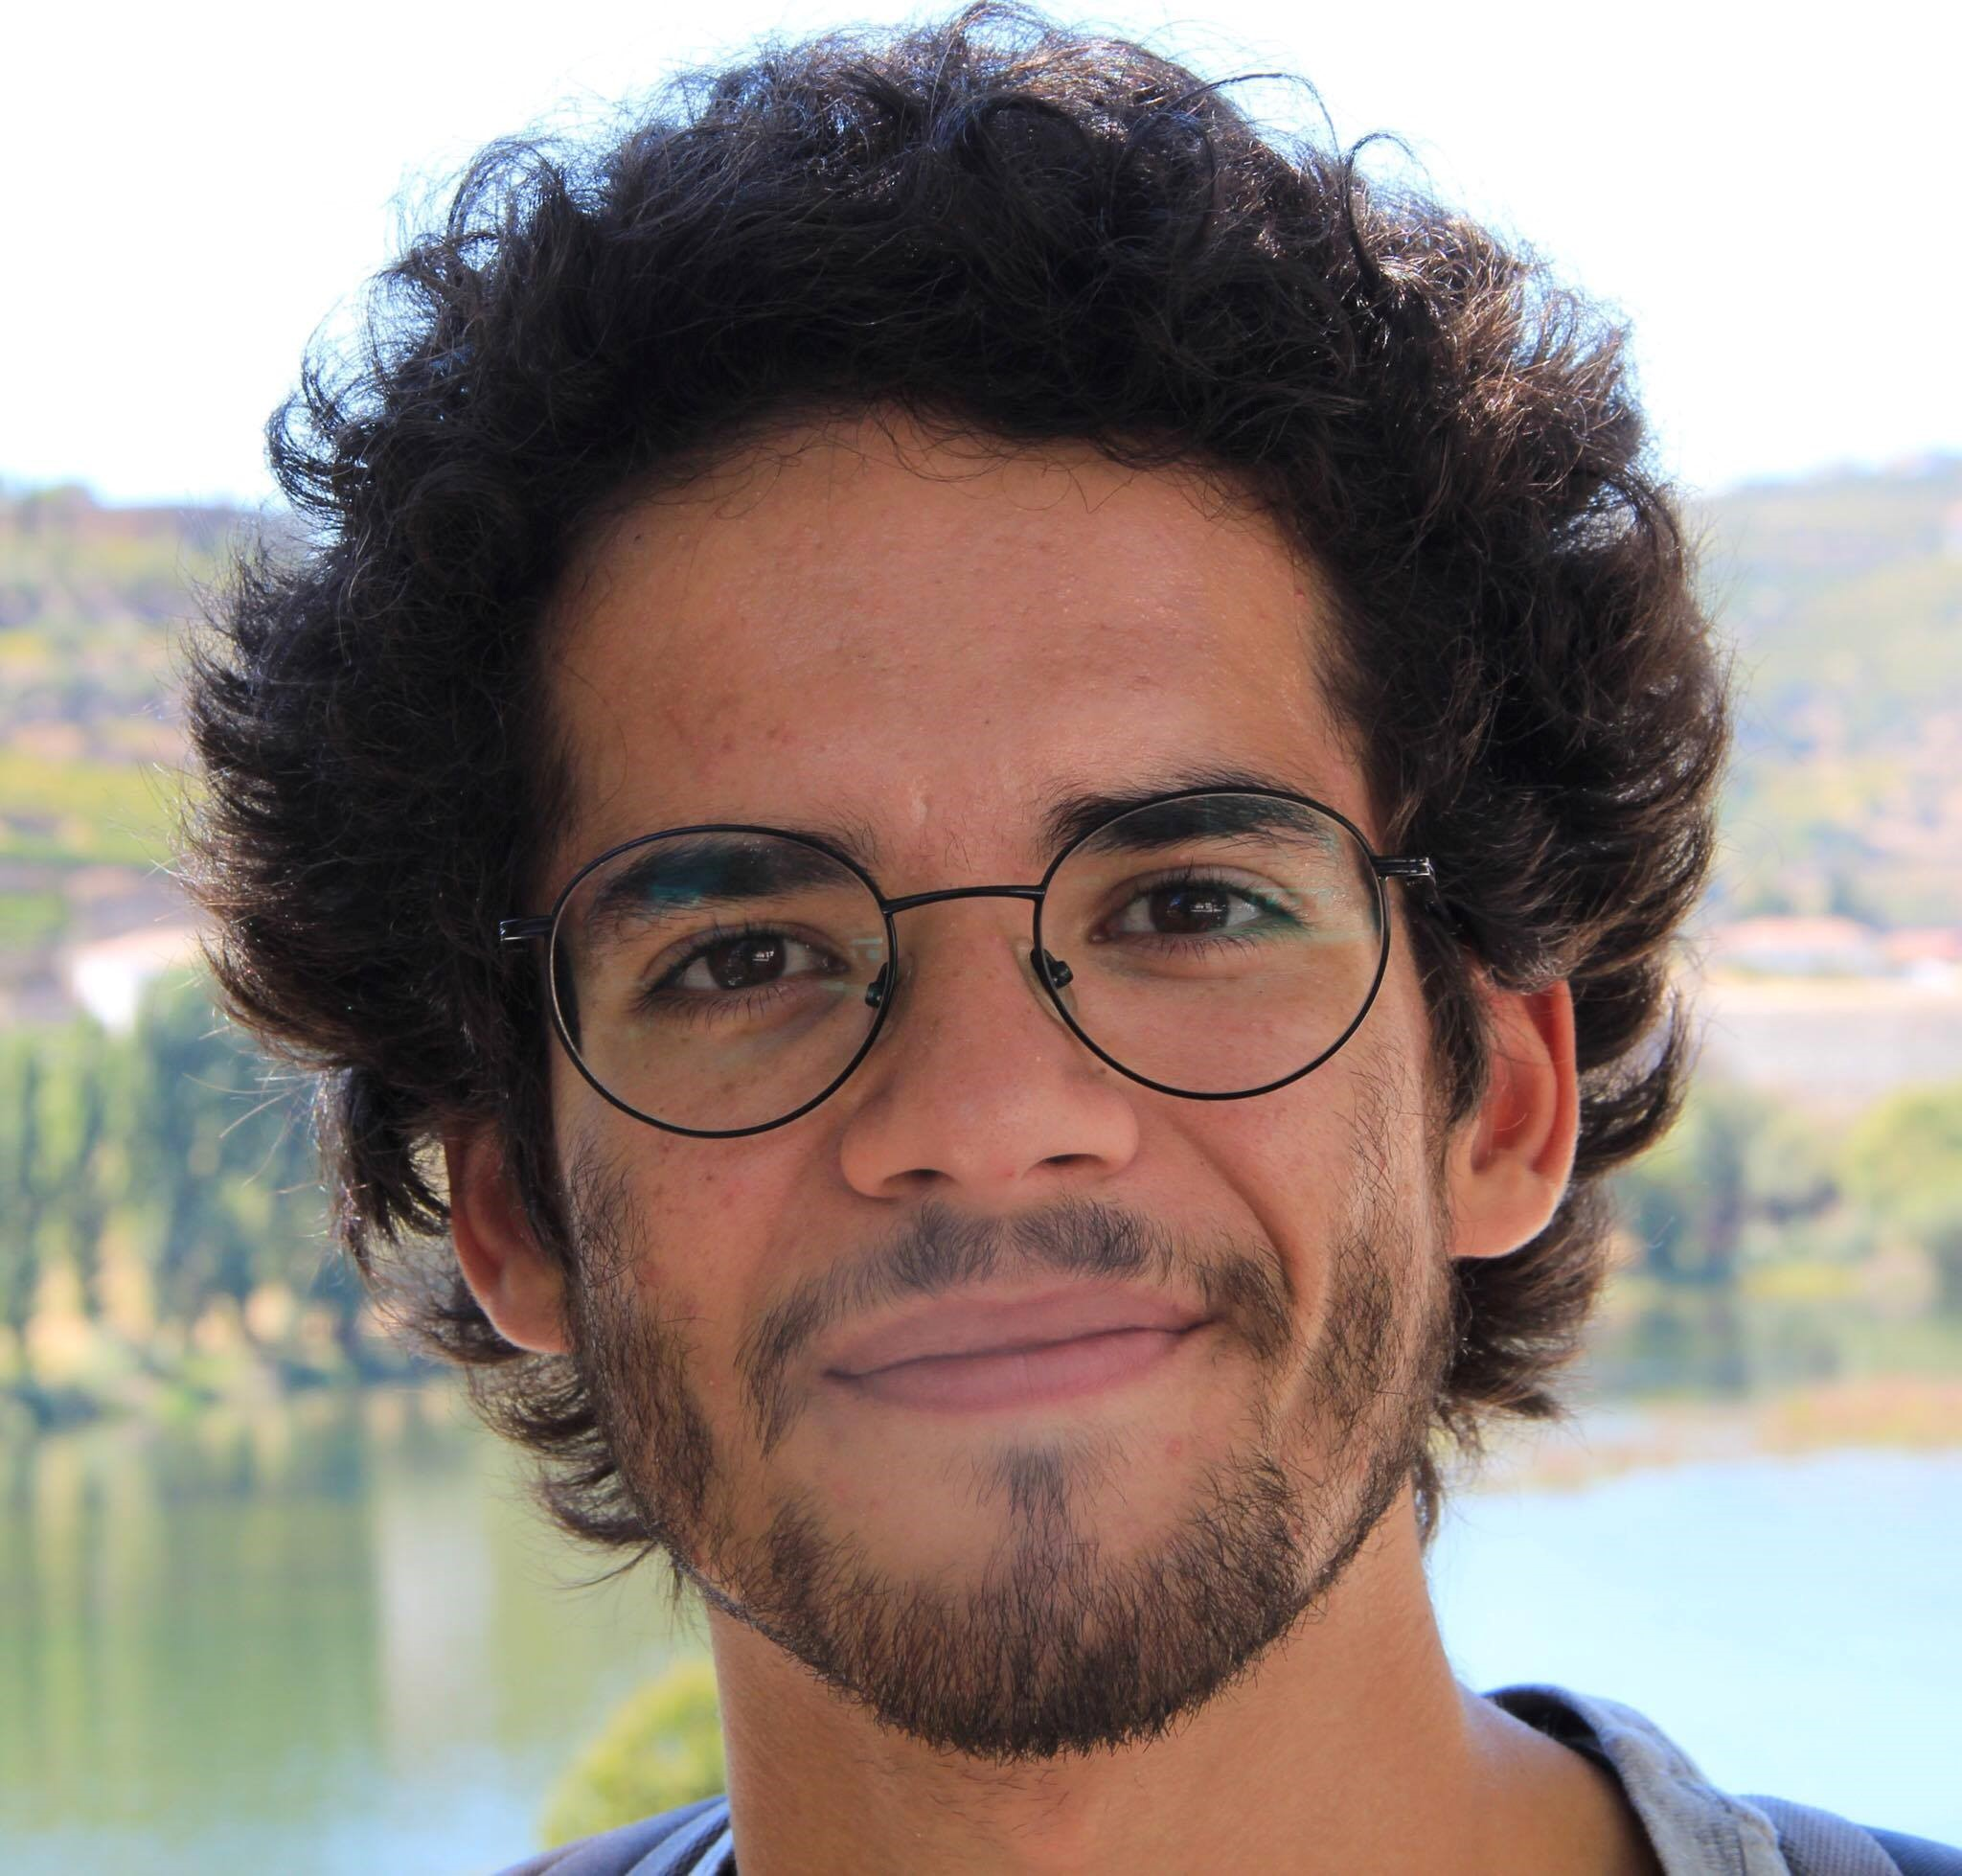
\includegraphics[width=1.5cm]{images/afonso} \end{array} $
    Diogo Costa \textsc{(A78034)}\\[0.3cm]
    $ \begin{array}{l} 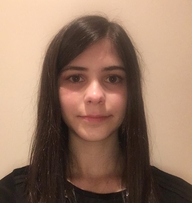
\includegraphics[width=1.5cm]{images/mafalda} \end{array} $
    Mafalda Nunes \textsc{(A77364)}\\[0.3cm]
    $ \begin{array}{l} 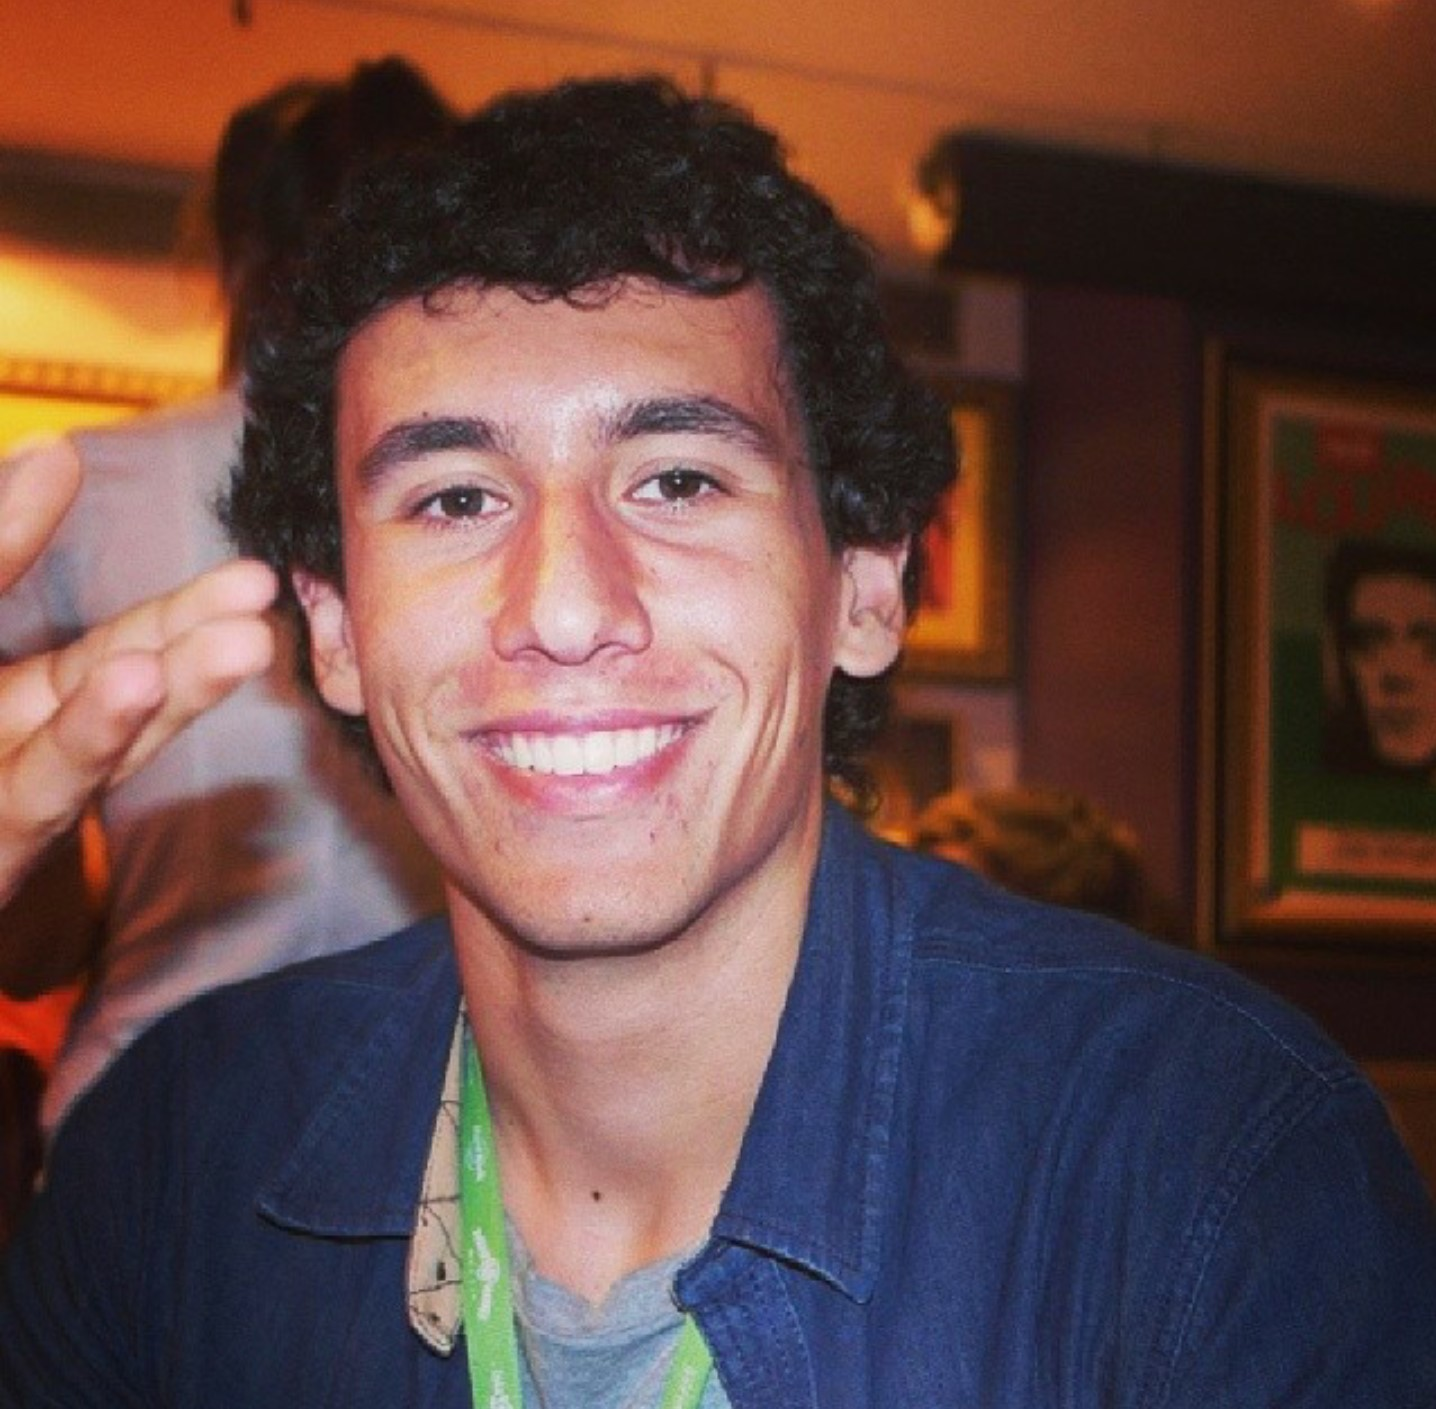
\includegraphics[width=1.5cm]{images/marco} \end{array} $
    Marco Silva \textsc{(A79607)}\\[0.3cm]
    $ \begin{array}{l} 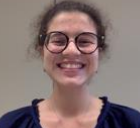
\includegraphics[width=1.5cm]{images/patricia} \end{array} $
    Patrícia Barreira \textsc{(A79007)}\\[0.3cm]
  \end{flushleft}
\end{minipage}%
\vfill

% Bottom of the page
{\large Versão 1.0 \\[0.2cm] \today}

\end{center}
\end{titlepage}


\begin{abstract}
O projeto \texttt{Home4All} constitui um \textit{website} que pretende oferecer funcionalidades relacionadas com o setor imobiliário, nomeadamente a compra e/ou venda de imóveis. 

Desta forma, começou-se por efetuar uma análise de requisitos na qual foram identificadas todas as funcionalidades do projeto, os utilizadores alvo e descritas as principais tarefas que compõem o sistema.

De seguida, passou-se para a modelação do sistema, onde foi elaborado o modelo de domínio, o \textit{mockup} da interface, com consequente avaliação ada usabilidade.

A terceira etapa, envolveu a implementação do projeto propriamente dito, através de uma abordagem baseada em modelos.

Por fim, foi realizado o \textit{deploy} da infraestrutura final em máquinas físicas, as quais foram submetidas a testes de carga com o objetivo de avaliar a performance do sistema.
\end{abstract}

\pagebreak
\tableofcontents


\pagebreak
\section{Introdução}
\label{sec:introducao}
\subfile{sections/introducao}

\pagebreak
\section{Contextualização}
\label{sec:contextualizacao}
\subfile{sections/contextualizacao}

\pagebreak
\section{Análise de Requisitos}
\label{sec:requisitos}
\subfile{sections/requisitos}

\pagebreak
\section{Domínio do Problema}
\label{sec:dominio}
\subfile{sections/dominio}

\pagebreak
\section{Concepção (Prototipagem)}
\label{sec:concepcao}
\subfile{sections/concepcao}

\pagebreak
\section{Desenvolvimento}
\label{sec:desenvolvimento}
\subfile{sections/desenvolvimento}

\pagebreak
\section{Conclusões}
\label{sec:conclusoes}
\subfile{sections/conclusoes}

\end{document}